\documentclass{article}

\usepackage{hyperref}          % Clickable link
\usepackage{indentfirst}

% References
\usepackage{biblatex}
\addbibresource{references.bib}

\usepackage{graphicx}          % Load images
\usepackage{float}             % Insert images at the current position using [h]
\graphicspath{ {./images/} }


\author{Nguyễn Việt Minh Nghĩa \\ \href{mailto:nvmnghia@gmail.com}{nvmnghia@gmail.com}}

\date{11/03/2020}

\title{Kiến trúc hướng dịch vụ INT3505 \\ Bài tập lớn số một \\ Tìm hiểu các mô hình của điện toán đám mây}

\begin{document}

\maketitle

\section{Định nghĩa}

\subsection{Tiền đề}

"Cloud computing" là chủ đề nhận được rất nhiều sự quan tâm trong ngành công
nghệ thông tin. Từ khóa này thậm chí vượt ra khỏi chuyên ngành, trở thành một
buzzword thông dụng. Giống với nhiều thuật ngữ lớn khác như AI, Big data, điện
toán đám mây không có một định nghĩa cụ thể và thống nhất.

Với lập trình viên, điện toán đám mây đưoc hiểu đơn giản là việc \emph{cung cấp
tài nguyên tính toán và lưu trữ qua mạng}. Để hiểu phần nào định nghĩa này, ta
cần so sánh cách điện toán đám mây với cách sử dụng truyền thống tài nguyên máy
tính.

Trước đây, hai loại tài nguyên này thường đưọc đặt \emph{tại địa điểm} phát
triển hoặc sử dụng (on-premise). Việc đặt tài nguyên máy tính tại địa điểm xuất
phát từ nhu cầu thiết yếu về mặt quản trị, bảo mật (giữ quyền kiểm soát vật lý),
nhưng cũng có lí do về giới hạn công nghệ (tài nguyên đặt ở xa thì sử dụng chậm
hơn). Điều này dẫn tới việc đến hai hậu quả:

\begin{itemize}
    \item Công ty phải trả phí cho rất nhiều dịch vụ đi kèm, chủ yếu gồm lắp đặt
    và bảo trì.
    \item Người dùng trực tiếp (người lập trình, người vận hành) phần nào vẫn
    phải bận tâm đến những vấn đè ngoài chuyên môn (bảo trì, sử dụng).
\end{itemize}

Cả công ty và người sử dụng đều mất tiền và thời gian, công sức không cần thiết.
Nói ngắn gọn, bài toán thực tế đặt ra là tài nguyên cần đưọc cung cấp mà người
dùng chỉ cần sử dụng trực tiếp, không phải lo việc bảo trì. Điện toán đám mây là
một lời giải cho nhu cầu này.

Điện toán đám mây bắt nguồn từ ý tưởng rằng vị trí và các hoạt động bảo trì của
tài nguyên cần \emph{trong suốt với với ngưòi dùng}, bằng cách đặt chúng trên
máy chủ \cite{SES2006}. Ý tưởng này giải quyết được cả hai vấn đề đề cập ở trên:

\begin{itemize}
    \item Ngưòi dùng chỉ cần kết nối đến máy chủ đó để truy cập và sử dụng tài
    nguyên, không cần quan tâm đến các công việc bảo trì như trước.
    \item Công ty chỉ cần trả chi phí định kì; phí này bao gồm tất cả chi phí
    mua sắm, vận hành, nâng cấp.
\end{itemize}

Với ý tưởng này, tài nguyên tính toán và lưu trữ trở thành một loại dịch vụ thuê
bao, giống với nước, điện và sóng điện thoại. Tổng chi phí sở hữu (total cost of
ownership - TCO) của doanh nghiệp được cắt giảm hoàn toàn, thay vào đó là phí
thuê bao. Cùng với điện, nước, điện toán đám mây có chi phí sử dụng không quá
đắt, do nhà cung cấp đã tối ưu được chi phí đầu tư thông qua việc mua sắm hạ
tầng với số lượng lớn.

Vấn đề với cách hiểu trên là sự thiếu chính xác, thể hiện ở một số điểm sau:

\begin{itemize}
    \item Thiếu tính hàn lâm
    \item Không phân biệt rõ ràng điện toán đám mây với một số dịch vụ đã từng
    tồn tại trước đó như máy chủ riêng áo (VPS), điện toán lưới (grid computing)
    \item Khó tránh bị lạm dụng trong quảng cáo
    \begin{itemize}
        \item Nhiều công ty, chủ yếu trong ngành dịch vụ máy chủ và ERP, trong
        đó có Dell, IBM, Oracle, dán mác "đám mây" cho các sản phẩm cũ của họ
        (cloudwashing) \cite{MITTR2011}.
        \item  Dell từng cố đăng kí bản quyền cụm từ "điện toán đám
        mây".
    \end{itemize}
\end{itemize}

Do vậy, cần thiết có một định nghĩa chính xác về điện toán đám mây. Phần tiếp
theo trình bày một định nghĩa như vậy của NIST, được công nhận và trích dẫn rộng
rãi, ra đời 5 năm sau khi điện toán đám mây trở nên phổ biến.

\subsection{Định nghĩa của NIST}

NIST định nghĩa điện toán đám mây như sau \cite{NIST2011}:

Điện toán đám mây là mô hình cho phép truy cập một cách thuận tiện, theo yêu cầu
vào một bể tài nguyên dùng chung. Tài nguyên đó có thể là mạng, máy chủ, thiết
bị lưu trữ, ứng dụng, dịch vụ. Tài nguyên này có thể được cấu hình, có thể được
cung cấp và hoàn trả nhanh chóng mà không cần can thiệp từ nhà cung cấp dịch vụ.
Mô hình này gồm năm đặc tính:

\begin{itemize}
    \item Tự phục vụ theo nhu cầu: Người dùng có thể sử dụng tài nguyên theo nhu
    cầu mà không cần liên hệ trước với nhà cung cấp dịch vụ.
    \item Truy cập qua mạng: Tài nguyên có thể đưọc sử dụng qua mạng, bằng các
    thiết bị đầu cuối thông thường, từ điện thoại đến máy tính.
    \item Tài nguyên dùng chung: Tài nguyên của nhà cung cấp đưọc gộp lại và cho
    mọi người dùng chung, sao cho sự riêng tư vẫn được đảm bảo. Dịch vụ cần đạt
    đưọc sự trong suốt về vị trí, theo nghĩa là người dùng không cần kiểm soát
    hay biết vị trí địa lí của tài nguyên, nhưng có thể chỉ định vị trí ở mức
    cao hơn (quốc gia, địa điểm, trung tâm dữ liệu,...).
    \item Cung cấp tài nguyên linh hoạt: tài nguyên có thể được cung cấp cho
    người dùng một cách tự động, không cần người dùng biết, tùy theo mức tải.
    Với người dùng, dịch vụ trông gần như vô tận.
    \item Dịch vụ được điều tiết: Hệ thống tự động điều khiển và tối ưu việc sử
    dụng tài nguyên bằng các công cụ đo lường. Chi phí sử dụng được tính theo
    các thông số đo đạc này. Các thông số có thể là số server sử dụng, giống như
    nhiều dịch vụ trước đó, nhưng cũng có thể là những thông số kĩ thuật như số
    CPU, IOPS,... Thông tin sử dụng có thể đưọc theo dõi, báo cáo cho cả người
    dùng và nhà cung cấp dịch vụ.
\end{itemize}

\section{Phân loại điện toán đám mây}

Tiếp nối phần một, phần này trình bày hai cách phân loại theo định nghĩa của
NIST.

\subsection{Phân loại theo mô hình dịch vụ}

Phân loại theo mô hình dịch vụ là cách phân loại điện toán đám mây phổ biến hơn
cả. Cách phân loại này chia điện toán đám mây ra ba mô hình:

\begin{itemize}
    \item Phần mềm dạng dịch vụ (SaaS)
    \item Nền tảng dạng dịch vụ (PaaS)
    \item Hạ tầng dạng dịch vụ (IaaS)
\end{itemize}

Hiểu đơn giản, XaaS - X dạng dịch vụ - nghĩa là dịch vụ đó cung cấp X, và X chạy
trên hạ tầng nhà cung cấp. Ví dụ, một dịch vụ được phân loại vào SaaS nghĩa là
dịch vụ đó cung cấp phần mềm, và phần mềm đó chạy trên hạ tầng máy tính của nhà
cung cấp, chứ không phải nhà cung cấp đó bán phần mềm, rồi cho phép người dùng
tự chọn nơi chạy. Từ "dịch vụ" là từ khóa quan trọng để hiểu XaaS. Thứ được cung
cấp không phải hàng hóa nói chung, vì nó không hoàn toàn thuộc sở hữu của người
mua.

Cách phân loại này dựa trên điểm nhìn của người sử dụng dịch vụ. Cụ thể hơn, nó
dựa vào việc phân mức các quyền người dùng được làm với dịch vụ (gồm cả phần mềm
và hạ tầng phần cứng) của nhà cung cấp dịch vụ điện toán đám mây. Nói cách khác,
đây vừa là kiểu phân loại, vừa là kiểu phân cấp. Hình \ref{csaguidev3} cho thấy
mức độ quyền của người dùng với ba mô hình.

\begin{figure}[H]
    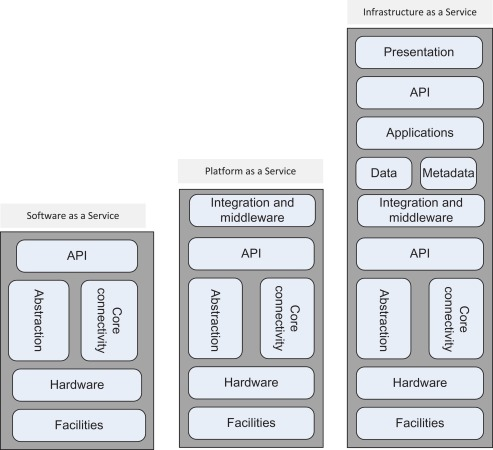
\includegraphics[scale=0.8]{csaguidev3.jpg}
    \centering
    \caption{Bậc tự do của ba mô hình dịch vụ \cite{CSA2011}.}
    \label{csaguidev3}
\end{figure}

\subsubsection{Phần mềm dạng dịch vụ}

Trong mô hình phần mềm dạng dịch vụ (Software as a Service - SaaS), người dùng
được truy cập phần mềm của nhà cung cấp, chạy trên hạ tầng của nhà cung cấp.
Người dùng không phải quan tâm về hạ tầng và phần mềm, chỉ đơn thuần sử dụng
dịch vụ. Ví dụ điển hình của loại dịch vụ này là Office 365, Google Apps (dù
được cung cấp miễn phí, Google có cách kiếm tiền riêng).

Phần mềm được cung cấp không chỉ là phần mềm viết riêng của nhà cung cấp dịch
vụ, mà còn có thể là phần mềm từ một hãng thứ ba. Ví dụ cho trường hợp này là
dịch vụ chạy SAP HANA trên AWS.

Dịch vụ dạng SaaS thường có khả năng truy cập nhanh bằng đại đa số các thiết bị
có kết nối mạng. Điều này nhìn chung là đúng với cả ba mô hình dịch vụ (do việc
xử lí nặng nề được chuyển về máy chủ), tuy nhiên SaaS có lợi thế là giảm tối đa
can thiệp của người dùng, chỉ tập trung vào trải nghiệm, do đó số loại thiết bị
có thể truy cập thuận tiện tăng lên đáng kể, bao gồm cả điện thoại thông minh.

Các loại dịch vụ SaaS có thể chia tiếp làm hai loại:

\begin{itemize}
    \item Dịch vụ cho tập đoàn: CRM, quản lí tài chính/thuế,...
    \item Ứng dụng Web 2.0: mạng xã hội, blog,...
\end{itemize}

\subsubsection{Hạ tầng dạng dịch vụ}

Ở thái cực ngược lại với SaaS, hạ tầng dạng dịch vụ (Infrastructure as a Service
- IaaS) cho phép người dùng can thiệp khá sâu vào hạ tầng phần mềm (hệ điều
hành). Hạ tầng phần cứng vẫn do phía nhà cung cấp kiểm soát, do đặc tính ở xa,
và đặc thù về cài đặt bên dưới (buộc phải sử dụng máy ảo, dẫn đến truy cập từ xa
vào phần cứng bị giới hạn).

Cụ thể hơn, người dùng được quyền chuẩn bị/cấp phát (provisioning) CPU, RAM, lưu
lượng mạng, và các tài nguyên cơ bản khác \cite{MARINESCU201813}, có thể chạy
bất kì phần mềm nào, bao gồm việc tùy chọn hệ điều hành để sử dụng. Quyền sử
dụng ở mức sâu này là điểm đặc thù của IaaS, giúp thu hút những công ty không
muốn đầu tư quá nhiều vào hạ tầng. Khả năng truy cập sâu này cũng cho phép người
dùng cài đặt tính năng tự động tăng giảm quy mô tính toán (auto-scaling).

Ví dụ đáng chú ý nhất của mô hình này là Amazon Web Service. Ra đời vào năm
2006, đồng thời là dịch vụ kích hoạt cuộc đua đám mây, đây luôn là dịch vụ đi
đầu, giúp thúc đấy sự phát triển của điện toán đám mây. Người dùng có rất nhiều
dịch vụ chuyên biệt để lựa chọn, trong đó quan trọng nhất là Elastic Compute
Cloud (EC2). EC2 cho phép người dùng chọn trước cấu hình của từng đơn vị máy chủ
(instance), cho phép chọn và cài lại hệ điều hành (machine image), và cung cấp
mọi quyền cấp hệ điều hành cho người dùng. EC2 có tính năng tự động tăng giảm
quy mô phần cứng (auto-scaling group, bằng việc tăng giảm số lượng instance).
Tính mềm dẻo, thể hiện cả trong auto-scaling lẫn việc tính toán thời gian dùng ở
mức chi tiết rất cao (thời gian sử dụng có thể tính theo giây), là điểm khiến
EC2 là dịch vụ khác biệt với các công nghệ trước đó, tại thời điểm ra mắt.

\subsubsection{Nền tảng dạng dịch vụ}

Ở mức giữa của IaaS và SaaS là nền tảng dạng dịch vụ (Platform as a Service). Mô
hình này cho phép người dùng chạy phần mềm và mã nguồn của riêng mình, nhưng bị
giới hạn một số cài đặt về môi trường. Tùy theo nhà cung cấp mà các giới hạn có
thể được nới lỏng hay thắt chặt, tuy nhiên một điểm chung đó là các dịch vụ PaaS
không cho phép tùy ý lựa chọn hệ điều hành. Thông thường, người dùng được tải
ứng dụng/mã nguồn của mình lên, và nó phải tương thích với môi trường (hệ điều
hành,...) đã chọn trước. Nhà cung cấp thường cung cấp một số thư viện riêng để
ứng dụng có thể làm việc tốt với môi trường đã chọn thay vì cho phép người dùng
cài đặt tùy thích các phần mềm bên thứ ba.

Ví dụ cho mô hình này là Google App Engine. App Engine cho phép người dùng tải
lên mã nguồn ở nhiều ngôn ngữ, có thư viện để lưu dữ liệu vào Bigtable/BigQuery
(thay cho các ứng dụng cơ sở dữ liệu OLTP/OLAP truyền thống), dùng ngôn ngữ truy
vấn riêng, và hạn chế truy cập vào hệ điều hành.

IaaS thường chính là nền tảng đầu tiên để các mô hình còn lại trong kiểu phân
loại này hoạt động.

\subsubsection{Mở rộng: FaaS và DBaaS}

Mở rộng định nghĩa XaaS, ta có thêm Function-aaS và Database-aaS. Hai loại hình
này không nằm trong phân loại của NIST (do không thể hiện tính phân quyền),
nhưng gần đây được nhắc đến nhiều do sự dễ dàng sử dụng. Cả hai đều ít nhiều
liên quan đến và/hoặc hay bị nhầm với PaaS.

"Hàm" trong hàm ở dạng dịch vụ có ý so sánh với hàm - khối logic nhỏ nhất trong
lập trình. FaaS thường có một số đặc điểm như sau:

\begin{itemize}
    \item Chỉ chấp nhận mã nguồn nhỏ gọn: FaaS cho phép kiểm soát môi trường ít
    hơn cả PaaS, có thể triển khai mà gần như không cần cấu hình.
    \item Kích hoạt khi cần: Ứng dụng không có process chờ kết nối mà được môi
    trường của nhà cung cấp kích hoạt khi cần.
\end{itemize}

Hai đặc điểm trên, đặc biệt là điểm thứ hai, dẫn đến khả năng auto-scaling vượt
trội của FaaS. Các đặc điểm này còn cho phép FaaS có cách tính phí đặc biệt, chỉ
tính lúc chương trình đang chạy (không tính ở chế độ chờ) và có độ chính xác đến
phần trăm giây, hoặc tính theo số lần sử dụng \cite{CFPvF}. Ví dụ tiêu biểu cho
mô hình này là Amazon Lambda, Azure Function. Gần đây, FaaS bắt đầu phổ biến,
gắn với kiến trúc serverless.

Cơ sở dữ liệu ở dạng dịch vụ là việc sử dụng cơ sở dữ liệu trên hạ tầng điện
toán đám mây. Đây có thể coi là một kiểu SaaS hơn là PaaS. Các dịch vụ DBaaS mới
(không đơn thuần là SaaS với phần mềm cơ sở dữ liệu có sẵn) như Google Bigtable
có nhiều tính năng, tiêu biểu như auto-scaling mà cơ sở dữ liệu thông thường
không có, hoặc phải cấu hình thủ công hay dùng phần mềm bên thứ ba, đồng thời
vẫn cung cấp các tính năng nâng cao truyền thống như sao lưu.

\subsection{Phân loại theo mô hình triển khai}

Tiếp tục theo cách phân loại của NIST, có bốn mô hình triển khai, phân loại dựa
vào độ riêng tư của môi trường.

\subsubsection{Điện toán đám mây dùng riêng}

Đây là mô hình có mức độ riêng tư, hiệu năng và bảo mật cao nhất. Trong mô hình
này, toàn bộ hạ tầng được dùng để phục vụ một tổ chức duy nhất. Hạ tầng có thể
được quản lí bởi một bộ phận hoặc bên thứ ba, có thể đặt tại công ty hoặc ở một
địa điểm khác, có thể là công ty tự mua và cài đặt hoặc thuê trọn gói một phần
của các nhà cung cấp dịch vụ lớn. Do chi phí đầu tư và quản lí quá lớn (kể cả
trong trường hợp dùng dịch vụ của các công ty lớn), một mạng đám mây riêng
thường yêu cầu chặt chẽ về mặt quy trình, được tích hợp tốt, dự đoán được các mở
rộng trong tương lai, thì mới có hiệu quả về mặt chi phí tổng thể so với việc
thuê thông thường.

Ví dụ về điện toán đám mây dùng riêng là Amazon Virtual Private Cloud - Amazon
cho thuê riêng các instance, cho người dùng nhiều quyền hơn cả gói IaaS thông
thường, tính bảo mật (cả phần mềm, phần cứng, vật lí) cao hơn, thậm chí cho phép
tùy biến. Bộ Quốc phòng Mỹ có gói thầu JEDI giá 10 tỉ USD để xây dựng nền tảng
điện toán đám mây dùng riêng mà Microsoft vừa thắng thầu. Nếu không có đủ chi
phí để tự thiết kế một hệ thống đám mây, tổ chức có thể tùy biến lại phần mềm từ
các dự án mã nguồn mở như OpenStack.

\subsubsection{Điện toán đám mây công cộng}

Trái ngược với mô hình riêng tư, mô hình công cộng cho phép mọi người cùng truy
cập vào bể tài nguyên chung. Khác biệt chính so với mô hình riêng tư chủ yếu là
ở độ bảo mật của dữ liệu.

Ví dụ về công ty theo mô hình điện toán đám mây công cộng là ba dịch vụ lớn:
Amazon Web Service, Microsoft Azure, Google Cloud Platform.

\subsubsection{Điện toán đám cộng đồng}

Đây là mô hình trung hòa giữa mô hình cộng đồng và mô hình riêng tư. Ở mô hình
này, một số tổ chức cùng nhau thuê hoặc mua thiết bị, cùng nhau quản lý hạ tầng
mạng. Ngoài việc nâng số tổ chức được dùng của mô hình riêng tư lên lớn hơn 1,
hai mô hình này cũng không khác gì nhau về mặt kĩ thuật.

\subsubsection{Điện toán đám mây lai}

Trong dạng này, hạ tầng đám mây có thể được kết hợp từ nhiều hơn một mô hình kể
trên. Tuy nhiên, hạ tầng đám mây không được gộp lại quản lí chung, mà "lai" ở
đây hiểu theo nghĩa các mạng thành phần có khả năng giao tiếp, chia sẻ với nhau.
Từng hạ tầng vẫn do tổ chức riêng quản lý, tuy nhiên trong trường hợp cần thiết
có thể chia sẽ tài nguyên cho nhau. Hạ tầng giao tiếp giữa các mạng thưòng rất
phức tạp, và có thể yêu cầu sự tương thích từ các phần mềm cốt lõi hẹ thống. Một
ví dụ cho khả năng của mô hình này là việc cân bằng tải giữa hai mô hình hạ tầng
khác nhau (sau cùng, hạ tầng đám mây cũng vẫn cung cấp tài nguyên tính toán và
lưu trữ).

\section{Phân tích khả năng sử dụng điện toán đám mây của Đại học Quốc gia Hà Nội}

\subsection{Bối cảnh}
Đại học Quốc gia Hà Nội có các cơ sở đào tạo tập trung trong nội thành Hà Nội,
có số sinh viên mỗi khóa từ 8000-10000. Lấy trung bình là 9000 một khóa, nhân
với 4 khóa, cộng thêm số học viên tốt nghiệp muộn, giảng viên, viên chức, hoặc
học chương trình sau đại học sẽ là khoảng 45000 người, tính dư thêm tránh nghẽn
là 50000. Trường có 10 khoa, 2 campus chính (Xuân Thủy và Nguyễn Trãi).

Hiện tại, ở Việt Nam đã có nhiều dịch vụ cung cấp hạ tầng điện toán đám mây
IaaS, tiêu biểu có Viettel IDC. IDC có trung tâm dữ liệu đặt ở Hòa Lạc, không xa
so với hai campus của trường. Tương lai trường sẽ chuyển hẳn lên Hòa Lạc, nếu sử
dụng dịch vụ của Viettel thì càng tiện lợi. Tuy nhiên, Viettel IDC nói riêng và
dịch vụ điện toán đám mây ở Việt Nam nói chung chưa có tính năng auto-scaling.

\subsection{Thực trạng}
Trong nhiều năm nay, nhu cầu sử dụng cao nhất của các học viên là hệ thống đăng
kí học, hệ thống website môn học hệ thống báo điểm và hệ thống thông tin thư
viện, với các kiểu tải khác nhau:

\begin{itemize}
    \item Hệ thống đăng kí học
        \begin{itemize}
            \item CCU \footnote{CCU: Concurrent users - Số người dùng cùng
            lúc.}: 1000-5000 tùy trường
                \begin{itemize}
                    \item Từng trường có thời gian đăng kí khác nhau, nên CCU
                    không quá lớn, nhưng luôn ở mức tối đa tùy trường.
                \end{itemize}
            \item Thời lượng tải: 2-4 giờ mỗi học kì, vào một ngày xác định (tùy
            trường)
            \item Đặc điểm phiên sử dụng:
                \begin{itemize}
                    \item Dữ liệu ít, đơn giản (chỉ gửi request JSON nhẹ).
                    \item Chất lượng dịch vụ có yêu cầu cao (không mất dữ liệu
                    đã đăng kí).
                \end{itemize}
            \item \textbf{Thực trạng}: Luôn quá tải
                \begin{itemize}
                    \item Thời gian tải lâu.
                    \item Kết nối và dữ liệu thường xuyên bị mất.
                \end{itemize}
        \end{itemize}
    \item Hệ thống website môn học
        \begin{itemize}
            \item CCU: 50-1000
            \item Thời lượng tải: tập trung vào 1h cuối ngày (deadline nộp bài)
            \item Đặc điểm phiên sử dụng:
                \begin{itemize}
                    \item Tải xuống không nhiều (tải tài liệu PDF nhẹ rải rác cả
                    ngày).
                    \item Tải lên tập trung vào cuối ngày (sinh viên nộp bài
                    tập).
                \end{itemize}
            \item \textbf{Thực trạng}: Ổn định, hơi chậm
        \end{itemize}
    \item Hệ thống thông tin thư viện
        \begin{itemize}
            \item CCU: 50-5000 mỗi thư viện (có hai thư viện chính)
            \item Thời lượng tải: tăng dần trong kì học, đạt đỉnh vào một tháng
            diễn ra kì thi
            \item Đặc điểm phiên sử dụng:
                \begin{itemize}
                    \item Phiên phức tạp (tìm kiếm trong cơ sở dữ liệu lớn).
                    \item Dữ liệu nặng (file PDF khá nặng, chưa kể PDF scan).
                \end{itemize}
            \item \textbf{Thực trạng}: Chậm
        \end{itemize}
    \item Hệ thống báo điểm
        \begin{itemize}
            \item CCU: 2000-5000 (thời gian báo điểm của các trường sát nhau)
            \item Thời lượng tải: một tháng sau thi
            \item Đặc điểm phiên sử dụng:
                \begin{itemize}
                    \item Nhiều người cùng chờ điểm.
                    \item File PDF điểm khá nhẹ.
                \end{itemize}
            \item \textbf{Thực trạng}: Chậm
        \end{itemize}
\end{itemize}

Đặc biệt, trong mùa dịch (tình huống đặc biệt, rất hiếm khi xảy ra), nhu cầu sử
dụng website môn học tăng, nhưng không tăng đột biến, với hai lí do như sau:

\begin{itemize}
    \item Nhiều kênh liên lạc khác phổ biến hơn (Facebook, Zalo).
    \item Chức năng đặc biệt tốn tài nguyên là stream bài dạy thì không được ưa
    chuộng (dùng Skype/Zoom).
\end{itemize}

Các hệ thống còn lại của trường chỉ có hệ thống quản lí sinh viên là có tầm quan
trọng đáng kể. Hệ thống này chỉ dành cho một số cán bộ quản lí.

\subsection{Phân tích}

\subsubsection{Hệ thống đăng kí học và Hệ thống báo điểm}

Do đặc điểm tải tăng mạnh nhưng lại dự đoán được thời điểm, đây là hệ thống lí
tưởng để triển khai trên hạ tầng điện toán đám mây. Với nguồn thu tăng (tăng học
sinh, tăng học phí, có chương trình thông tư 32), tải có sự phân cực rõ rệt,
đồng thời thời gian đạt đỉnh rất ngắn, việc đưa hệ thống này lên mây là nhu cầu
bức thiết của sinh viên. Nhìn chung đây cũng là vấn đề của đại đa số đại học
trên cả nước, nếu thực hiện tốt sẽ tạo hình ảnh tích cực về trường.

\subsubsection{Hệ thống thông tin thư viện}

Hệ thống này có nhu cầu cao vào khoảng cuối kì, có thể nói là dự đoán được thời
điểm, nhưng số CCU vẫn khó dự đoán. Lượng dữ liệu lớn, truy vấn không đơn giản.
Hệ thống này có thể được đưa lên mây, tuy nhiên cần cân nhắc kĩ chi phí.

\subsection{Hệ thống website môn học}

Hệ thống này không có tải cao rõ rệt. Với chất lượng ổn định, hệ thống này không
cần thiết phải đưa lên mây.

\subsection{Hệ thống quản lí sinh viên}

Hệ thống quản lí sinh viên có đặc thù chỉ dành cho các cán bộ quản lí, đồng thời
yêu cầu cao về bảo mật. Hiện tại, hệ thống được đặt trong máy chủ ở trường, vừa
đảm bảo tính bảo mật, vừa đảm bảo tốc độ truy cập nhanh cho công tác quản lí. Hệ
thống này không cần đưa lên mây vì hiện tại đủ tốt, tuy nhiên cần có hệ thống
sao lưu dữ liệu thường xuyên, một số nhà cung cấp dịch vụ điện toán đám mây ở
Việt Nam đã hỗ trợ dịch vụ lưu trữ lâu dài cần thiết cho sao lưu.

\printbibliography

\end{document}
